\section{Nichtlineare Gleichungen}

%\subsection{Einleitung}

\subsection{Einfache Verfahren und ihre geometrische Interpretation}
\subsubsection{Bisektions-Verfahren}

% \begin{defi}{Einschließungsverfahren}
%     Verfahren, die untere und obere Schranken $a_k$ und $b_k$ für eine gesuchte Nullstelle erzeugen, nennt man \emph{Einschließungsverfahren}.
% \end{defi}

\begin{defi}{Bisektions-Verfahren}
    Wir setzen $f: \R \to \R$ stetig voraus.
    
    Ist $f(a_0) \cdot f(b_0) < 0$, dann muss in $[a_0, b_0]$ \emph{mindestens} eine Nullstelle von $f$ liegen.
    
    Betrachte $x_0 = \frac{a_0 + b_0}{2}$, also die Intervallmitte.
    
    Wiederhole solange, bis die Intervalllänge $|b_i - a_i|$ oder $|f(x_i)|$ hinreichend klein ist:
    \begin{itemize}
        \item Berechne
              \[
                  x_{i} = \frac{a_i + b_i}{2}
              \]
        \item Setze
              \[
                  \begin{cases}
                      a_{i+1} = a_{i}, \quad b_{i+1} = x_{i} & \text{falls } f(a_{i}) \cdot f(x_{i}) < 0 \\
                      a_{i+1} = x_{i}, \quad b_{i+1} = b_{i} & \text{sonst}
                  \end{cases}
              \]
        \item Betrachte nun $[a_{i+1}, b_{i+1}]$
    \end{itemize}
    
    Das Bisektions-Verfahren ist ein Einschließungsverfahren.
\end{defi}

\begin{example}{Bisektions-Verfahren}
    Gegeben sei die Funktion $f(x)$ und das Intervall $[a_0, b_0]$ mit: 
    \[ 
        f(x) = x^2 - 3, \quad a_0 = 0, \quad b_0 = 2
    \]
    
    Führen Sie das Bisektions-Verfahren durch.
    
    \exampleseparator
    
    $k = 0$:
    \[ 
        x_0 = \frac{a_0 + b_0}{2} = \frac{0 + 2}{2} = 1
    \]
    \[ 
        f(a_0) \cdot f(x_0) = -3 \cdot (-2) = 6 \geq 0 \quad \implies \quad a_1 = x_0 = 1, \quad b_1 = b_0 = 2
    \]
    
    $k = 1$:
    \[ 
        x_1 = \frac{a_1 + b_1}{2} = \frac{1 + 2}{2} = \frac{3}{2}
    \]
    \[ 
        f(a_1) \cdot f(x_1) = -2 \cdot \left(-\frac{3}{4}\right) = \frac{3}{2} \geq 0 \quad \implies \quad a_2 = x_1 = \frac{3}{2}, \quad b_2 = b_1 = 2
    \]
    
    $k = 2$:
    \[ 
        x_2 = \frac{a_2 + b_2}{2} = \frac{\frac{3}{2} + 2}{2} = \frac{7}{4}
    \]
    \[ 
        f(a_2) \cdot f(x_2) = \frac{1}{16} \cdot 1 = -\frac{1}{16} < 0 \quad \implies \quad a_3 = a_2 = \frac{3}{2}, \quad b_3 = x_2 = \frac{7}{4}
    \]
    
    usw.
    
    \begin{center}
        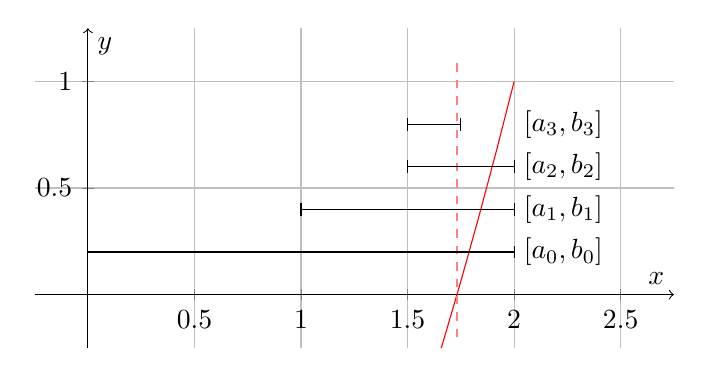
\begin{tikzpicture}
            \begin{axis}[
                    % xtick distance=2,
                    % ytick distance=2,
                    grid=major,
                    % grid style={line width=.1pt, draw=gray!10}%,major grid style={line width=.2pt,draw=gray!50}
                    % ticks=none, % ticks aus?
                    axis lines = middle,
                    axis line style={->},
                    ymin=-0.25, ymax=1.25,
                    xmin=-0.25, xmax=2.75,
                    xlabel={$x$},
                    ylabel={$y$},
                    axis equal image,
                    width=0.8\textwidth,
                    domain=0:2,
                ]
                % f = x^2-3
                \addplot[no marks, red]{x^2-3};
                \draw[red!50, dashed] (axis cs:1.73205,-0.2) -- (axis cs:1.73205,1.1);
                
                
                \draw (axis cs:0,0.2) -- (axis cs:2,0.2);
                \draw (axis cs:0,0.17) -- (axis cs:0,0.23);
                \draw (axis cs:2,0.17) -- (axis cs:2,0.23);
                
                \draw (axis cs:1,0.4) -- (axis cs:2,0.4);
                \draw (axis cs:1,0.37) -- (axis cs:1,0.43);
                \draw (axis cs:2,0.37) -- (axis cs:2,0.43);
                
                \draw (axis cs:1.5,0.6) -- (axis cs:2,0.6);
                \draw (axis cs:1.5,0.57) -- (axis cs:1.5,0.63);
                \draw (axis cs:2,0.57) -- (axis cs:2,0.63);
                
                \draw (axis cs:1.5,0.8) -- (axis cs:7/4,0.8);
                \draw (axis cs:1.5,0.77) -- (axis cs:1.5,0.83);
                \draw (axis cs:7/4,0.77) -- (axis cs:7/4,0.83);
                
                
                % labels
                \node[right] at (axis cs:2,0.2) {$[a_0, b_0]$};
                \node[right] at (axis cs:2,0.4) {$[a_1, b_1]$};
                \node[right] at (axis cs:2,0.6) {$[a_2, b_2]$};
                \node[right] at (axis cs:2,0.8) {$[a_3, b_3]$};
            \end{axis}
        \end{tikzpicture}
    \end{center}
\end{example}

\subsubsection{Regula-Falsi-Verfahren}

\begin{bonus}{Regula-Falsi-Verfahren (Idee)}
    Wir modifizieren das Bisektions-Verfahren, um die Konvergenzgeschwindigkeit zu erhöhen.
    
    Benutze für $x_k$ nicht die Intervallmitte, sondern zusätzliche Information:
    \begin{itemize}
        \item verbinde $(a_k, f(a_k))$ und $(b_k, f(b_k))$ durch eine Gerade $s$
        \item $x_k$ sei jetzt die Nullstelle der Geraden $s$ mit
              \[
                  s(x) = f(a_k) + \frac{f(b_k) - f(a_k)}{b_k - a_k} \cdot (x - a_k)
              \]
              \[
                  s(x_k) = 0 \quad \iff \quad x_k = a_k - \frac{b_k - a_k}{f(b_k) - f(a_k)} = \frac{a_k f(b_k) - b_k f(a_k)}{f(b_k) - f(a_k)}
              \]
    \end{itemize}
\end{bonus}

\begin{defi}{Regula-Falsi-Verfahren}
    Das \emph{Regula-Falsi-Verfahren} funktioniert analog zum Bisektions-Verfahren, nur dass $x_k$ wie folgt berechnet wird:
    \[
        x_k = \frac{a_k f(b_k) - b_k f(a_k)}{f(b_k) - f(a_k)}
    \]
    
    Wiederhole solange, bis die Intervalllänge $|x_{i+1} - x_i|$ oder $|f(x_i)|$ hinreichend klein ist:\footnote{Anderes Abbruchkriterium als beim Bisektions-Verfahren!}
    \begin{itemize}
        \item Berechne
              \[
                  x_{i} = \frac{a_k f(b_k) - b_k f(a_k)}{f(b_k) - f(a_k)}
              \]
        \item Setze
              \[
                  \begin{cases}
                      a_{i+1} = a_{i}, \quad b_{i+1} = x_{i} & \text{falls } f(a_{i}) \cdot f(x_{i}) < 0 \\
                      a_{i+1} = x_{i}, \quad b_{i+1} = b_{i} & \text{sonst}
                  \end{cases}
              \]
        \item Betrachte nun $[a_{i+1}, b_{i+1}]$
    \end{itemize}
    
    Das Regula-Falsi-Verfahren ist ein Einschließungsverfahren.
\end{defi}

\begin{example}{Regula-Falsi-Verfahren}
    Gegeben sei die Funktion $f(x)$ und das Intervall $[a_0, b_0]$ mit: 
    \[ 
        f(x) = x^2 - 3, \quad a_0 = 0, \quad b_0 = 2
    \]
    
    Führen Sie das Regula-Falsi-Verfahren durch.
    
    \exampleseparator
    
    $k = 0$:
    \[ 
        x_{0} = \frac{a_0 f(b_0) - b_0 f(a_0)}{f(b_0) - f(a_0)} = \frac{0 - 2 \cdot (-3)}{1 - (-3)} = \frac{3}{2}
    \]
    \[ 
        f(a_0) \cdot f(x_0) = -3 \cdot \left(-\frac{3}{4}\right) = \frac{9}{4} \geq 0 \quad \implies \quad a_1 = x_0 = \frac{3}{2}, \quad b_1 = b_0 = 2
    \]
    
    $k = 1$:
    \[ 
        x_{1} = \frac{a_1 f(b_1) - b_1 f(a_1)}{f(b_1) - f(a_1)} = \frac{\frac{3}{2} \cdot 1 - 2 \cdot \left(-\frac{3}{4}\right)}{1 - \left(-\frac{3}{4}\right)} = \frac{12}{7}
    \]
    \[ 
        f(a_1) \cdot f(x_1) = -\frac{3}{4} \cdot \left(-\frac{3}{49}\right) = \ldots \geq 0 \quad \implies \quad a_2 = x_1 = \frac{12}{7}, \quad b_2 = b_1 = 2
    \]
    
    $k = 2$:
    \[ 
        x_{2} = \frac{a_2 f(b_2) - b_2 f(a_2)}{f(b_2) - f(a_2)} = \frac{\frac{12}{7} \cdot 1 - 2 \cdot \left(-\frac{3}{49}\right)}{1 - \left(-\frac{3}{49}\right)} = \frac{45}{26}
    \]
    \[ 
        f(a_2) \cdot f(x_2) = -\frac{3}{49} \cdot \left(-\frac{3}{676}\right) = \ldots \geq 0 \quad \implies \quad a_3 = x_2 = \frac{45}{26}, \quad b_2 = b_1 = 2
    \]
    
    usw.
    
    \begin{center}
        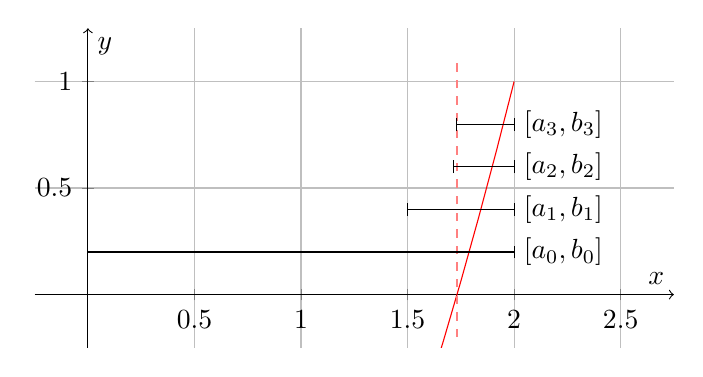
\begin{tikzpicture}
            \begin{axis}[
                    % xtick distance=2,
                    % ytick distance=2,
                    grid=major,
                    % grid style={line width=.1pt, draw=gray!10}%,major grid style={line width=.2pt,draw=gray!50}
                    % ticks=none, % ticks aus?
                    axis lines = middle,
                    axis line style={->},
                    ymin=-0.25, ymax=1.25,
                    xmin=-0.25, xmax=2.75,
                    xlabel={$x$},
                    ylabel={$y$},
                    axis equal image,
                    width=0.8\textwidth,
                    domain=0:2,
                ]
                % f = x^2-3
                \addplot[no marks, red]{x^2-3};
                \draw[red!50, dashed] (axis cs:1.73205,-0.2) -- (axis cs:1.73205,1.1);
                
                \draw (axis cs:0,0.2) -- (axis cs:2,0.2);
                \draw (axis cs:0,0.17) -- (axis cs:0,0.23);
                \draw (axis cs:2,0.17) -- (axis cs:2,0.23);
                
                \draw (axis cs:3/2,0.4) -- (axis cs:2,0.4);
                \draw (axis cs:3/2,0.37) -- (axis cs:3/2,0.43);
                \draw (axis cs:2,0.37) -- (axis cs:2,0.43);
                
                \draw (axis cs:12/7,0.6) -- (axis cs:2,0.6);
                \draw (axis cs:12/7,0.57) -- (axis cs:12/7,0.63);
                \draw (axis cs:2,0.57) -- (axis cs:2,0.63);
                
                \draw (axis cs:45/26,0.8) -- (axis cs:2,0.8);
                \draw (axis cs:45/26,0.77) -- (axis cs:45/26,0.83);
                \draw (axis cs:2,0.77) -- (axis cs:2,0.83);
                
                % labels
                \node[right] at (axis cs:2,0.2) {$[a_0, b_0]$};
                \node[right] at (axis cs:2,0.4) {$[a_1, b_1]$};
                \node[right] at (axis cs:2,0.6) {$[a_2, b_2]$};
                \node[right] at (axis cs:2,0.8) {$[a_3, b_3]$};
            \end{axis}
        \end{tikzpicture}
    \end{center}
\end{example}

\subsubsection{Sekanten-Verfahren}

\begin{defi}{Sekanten-Verfahren}
    Wir erhalten das \emph{Sekanten-Verfahren}, indem wir das Regula-Falsi-Verfahren leicht abändern.
    
    Seien $x_{-2}, x_{-1}$ gegeben.
    Bestimme für $k = 0, 1, \ldots$ die neue Näherung $x_k$ als Nullstelle der Geraden durch die Punkte
    \[
        x_k = x_{k-2} - \frac{x_{k-1} - x_{k-2}}{f(x_{k-1}) - f(x_{k-2})} \cdot f(x_{k-2}) = x_{k-1} - \frac{x_{k-1} - x_{k-2}}{f(x_{k-1}) - f(x_{k-2})} \cdot f(x_{k-1})
    \]
    
    Das Sekanten-Verfahren ist \emph{kein} Einschließungsverfahren.
\end{defi}

\begin{bonus}{Konvergenz des Sekanten-Verfahrens}
    Ist $f$ zweimal stetig differenzierbar in einer hinreichend kleinen Umgebung $X$ der gesuchten Nullstelle $x$.
    
    Dann konvergiert das Sekanten-Verfahren für alle $x_{-2}, x_{-1} \in X$ und es gibt eine Konstante $c > 0$ so dass
    \[
        |e_k| \leq c |e_{k-1}|^{\frac{1+\sqrt{2}}{2}}, \quad k \to \infty
    \]
\end{bonus}

\begin{example}{Sekanten-Verfahren}
    Gegeben sei die Funktion $f(x)$ und die Punkte $x_{-2}, x_{-1}$ mit: 
    \[ 
        f(x) = x^2 - 3, \quad x_{-2} = 0, \quad x_{-1} = 2
    \]
    
    Führen Sie das Sekanten-Verfahren durch.
    
    \exampleseparator
    
    $k = 0$:
    \[
        x_0 = x_{-1} - \frac{x_{-1} - x_{-2}}{f(x_{-1}) - f(x_{-2})} \cdot f(x_{-1}) = 2 - \frac{2 - 0}{1 - (-3)} \cdot 1 = \frac{3}{2}
    \]
    
    $k = 1$:
    \[
        x_1 = x_{0} - \frac{x_{0} - x_{-1}}{f(x_{0}) - f(x_{-1})} \cdot f(x_{0}) = \frac{3}{2} - \frac{\frac{3}{2} - 2}{-\frac{3}{4} - 1} \cdot \left(-\frac{3}{4}\right) = \frac{12}{7}
    \]
    
    $k = 2$:
    \[
        x_2 = x_{1} - \frac{x_{1} - x_{0}}{f(x_{1}) - f(x_{0})} \cdot f(x_{1}) = \frac{12}{7} - \frac{\frac{12}{7} - \frac{3}{2}}{-\frac{3}{49} - \left(-\frac{3}{4}\right)} \cdot \left(-\frac{3}{49}\right) = \frac{26}{15}
    \]
    
    usw.
    
    \begin{center}
        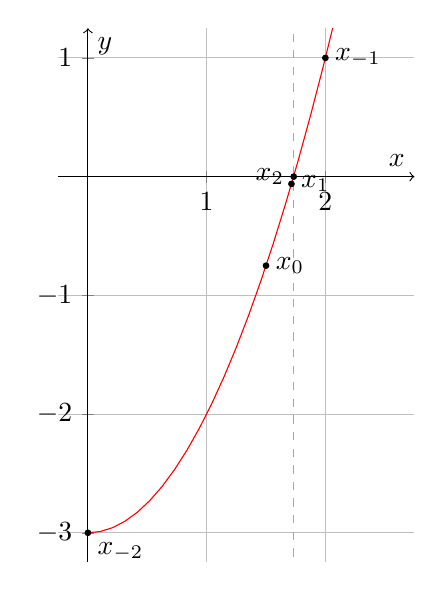
\begin{tikzpicture}
            \begin{axis}[
                    % xtick distance=2,
                    % ytick distance=2,
                    grid=major,
                    % grid style={line width=.1pt, draw=gray!10}%,major grid style={line width=.2pt,draw=gray!50}
                    % ticks=none, % ticks aus?
                    axis lines = middle,
                    axis line style={->},
                    ymin=-3.25, ymax=1.25,
                    xmin=-0.25, xmax=2.75,
                    xlabel={$x$},
                    ylabel={$y$},
                    axis equal image,
                    width=0.8\textwidth,
                    domain=0:2.5,
                ]
                % f = x^2-3
                \addplot[no marks, red]{x^2-3};
                \draw[red!50, dashed] (axis cs:1.73205,-3.2) -- (axis cs:1.73205,1.2);
                
                \draw[fill, black] (axis cs: 0, -3) circle (1pt) node[below right] {$x_{-2}$};
                \draw[fill, black] (axis cs: 2, 2^2-3) circle (1pt) node[right] {$x_{-1}$};
                \draw[fill, black] (axis cs: 3/2, 1.5^2-3) circle (1pt) node[right] {$x_{0}$};
                \draw[fill, black] (axis cs: 12/7, 1.7143^2-3) circle (1pt) node[right] {$x_{1}$};
                \draw[fill, black] (axis cs: 26/15, 0) circle (1pt) node[left] {$x_{2}$};
            \end{axis}
        \end{tikzpicture}
    \end{center}
\end{example}

\subsubsection{Taylor-Reihen-basierte Verfahren, Newton-Verfahren}

\begin{bonus}{Wiederholung Taylor-Entwicklung}
    Ist $f(x) = 0$ und $f$ hinreichend oft differenzierbar, $x_k$ gegeben, so liefert eine Taylor-Entwicklung von $f$ um $x_k$
    \[
        f(y) = f(x_k) + (y - x_k) f'(x_k) + \frac{(y - x_k)^2}{2!} f''(x_k) + \ldots
    \]
    bzw. für $y = x \implies f(y) = 0$
    \[
        0 = f(x) = f(x_k) + (x - x_k) f'(x_k) + \frac{(x - x_k)^2}{2!} f''(x_k) + \ldots
    \]
\end{bonus}

\begin{defi}{Newton-Verfahren (Tangente)}
    Brechen wir die Taylor-Entwicklung nach dem linearen Term ab, dann ist
    \[
        0 = f(x_k) + (\tilde{x} - x_k) f'(x_k) \quad \implies \quad \tilde{x} = x_k - \frac{f(x_k)}{f'(x_k)}
    \]
    und wir erhalten das \emph{Newton-Verfahren} mit
    \[
        x_{k+1} = x_k - \frac{f(x_k)}{f'(x_k)}
    \]
    
    Geometrisch approximiert das Newton-Verfahren also $f$ durch die Tangente $g$ durch den Punkt $(x_k, f(x_k))$ und benutzt die Nullstelle von $g$ als $x_{k+1}$.
\end{defi}

\begin{example}{Newton-Verfahren}
    Gegeben sei die Funktion $f(x)$ und der Punkt $x_{0}$ mit: 
    \[ 
        f(x) = x^2 - 3, \quad x_{0} = 1
    \]
    
    Führen Sie das Newton-Verfahren durch.
    
    \exampleseparator
    
    Es gilt: 
    \[ 
        f(x) = x^2 - 3 \quad \implies \quad f'(x) = 2x
    \]
    
    $k = 0$:
    \[
        x_{1} = x_0 - \frac{f(x_0)}{f'(x_0)} = 1 - \frac{-2}{2} = \frac{3}{2} = 1.5
    \]
    
    $k = 1$:
    \[
        x_{2} = x_1 - \frac{f(x_1)}{f'(x_1)} = \frac{3}{2} - \frac{-\frac{3}{4}}{3} = \frac{7}{4} = 1.75
    \]
    
    $k = 2$:
    \[
        x_{3} = x_2 - \frac{f(x_2)}{f'(x_2)} = \frac{7}{4} - \frac{\frac{1}{16}}{\frac{7}{2}} = \frac{97}{56} \approx 1.7321
    \]
    
    usw.
    
    \begin{center}
        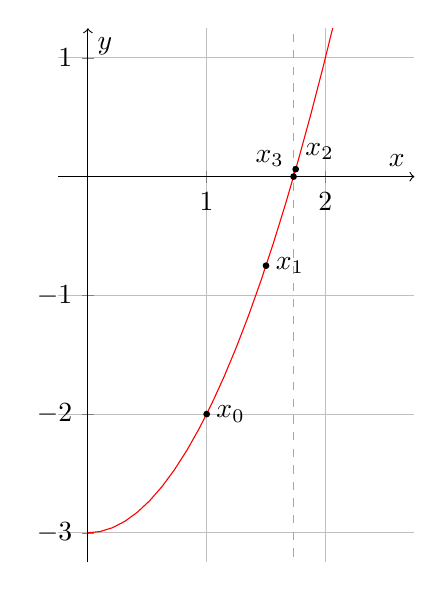
\begin{tikzpicture}
            \begin{axis}[
                    % xtick distance=2,
                    % ytick distance=2,
                    grid=major,
                    % grid style={line width=.1pt, draw=gray!10}%,major grid style={line width=.2pt,draw=gray!50}
                    % ticks=none, % ticks aus?
                    axis lines = middle,
                    axis line style={->},
                    ymin=-3.25, ymax=1.25,
                    xmin=-0.25, xmax=2.75,
                    xlabel={$x$},
                    ylabel={$y$},
                    axis equal image,
                    width=0.8\textwidth,
                    domain=0:2.5,
                ]
                % f = x^2-3
                \addplot[no marks, red]{x^2-3};
                \draw[red!50, dashed] (axis cs:1.73205,-3.2) -- (axis cs:1.73205,1.2);
                
                \draw[fill, black] (axis cs: 1, 1^2-3) circle (1pt) node[right] {$x_{0}$};
                \draw[fill, black] (axis cs: 1.5, 1.5^2-3) circle (1pt) node[right] {$x_{1}$};
                \draw[fill, black] (axis cs: 1.75, 1.75^2-3) circle (1pt) node[above right] {$x_{2}$};
                \draw[fill, black] (axis cs: 1.7321, 1.7321^2-3) circle (1pt) node[above left] {$x_{3}$};
            \end{axis}
        \end{tikzpicture}
    \end{center}
\end{example}

\begin{bonus}{Newton-Verfahren (Parabel)}
    Brechen wir nach dem quadratischen Term ab so folgt
    \[
        0 = f(x_k) + (\tilde{x} - x_k) f'(x_k) + \frac{(\tilde{x} - x_k)^2}{2} f''(x_k)
    \]
    und damit
    \[
        x_{k+1} = x_k - \frac{f'(x_k) \pm \sqrt{(f'(x_k))^2 - 2 \cdot f(x_k) f''(x_k)}}{f''(x_k)}
    \]
    
    Hier wird statt einer Tangente eine Parabel $g$ verwendet.
\end{bonus}

\subsection{Stationäre Iterationen, Banachscher Fixpunktsatz}

% \begin{defi}{Picard-Iteration}
%     TODO
% \end{defi}

\begin{defi}{Kontraktion}
    $\Phi$ heißt \emph{Kontraktion} bezüglich $\| \cdot \|$ auf $X \subset \R^n$ falls
    \begin{enumerate}
        \item $\Phi: X \to X$
        \item $\|\Phi(x) - \Phi(y)\| \leq \alpha \|x-y\|$, $\forall x, y \in X$ und $\alpha < 1$ unabhängig von $x, y$\footnote{Äquivalent: $\displaystyle \alpha \leq \max_{\zeta \in X} |\Phi'(\zeta)|$}
    \end{enumerate}
\end{defi}

\begin{example}{Kontraktion}
    Gegeben sei die Funktion $f(x) = x - e^{-x}$. 
    
    Zeigen Sie, dass das Newton-Verfahren $\Phi$ auf dem Intervall $X = [0, 1]$ konvergiert bzw. dass $\Phi$ eine Kontraktion auf $X$ ist.
    
    \exampleseparator
    
    Es gilt: 
    \[ 
        \Phi(x) = x - \frac{f(x)}{f'(x)} = x - \frac{x - e^{-x}}{1 + e^{-x}} = x - \frac{e^x \left(x - e^{-x}\right)}{e^x \left(1 + e^{-x}\right)} = \frac{x}{e^x + 1} - \frac{e^xx - 1}{e^x + 1} = \frac{x+1}{e^x + 1}
    \]
    
    $\Phi(x)$ ist eine Kontraktion, wenn: 
    \begin{itemize}
        \item $\Phi(x) \subset X \quad \iff \quad \forall x \in [0, 1]: \Phi(x) \in [0, 1]$:
              \begin{itemize}
                  \item Rand:
                        \[ \Phi(0) = \frac{1}{2} \in [0, 1], \quad \Phi(1) = \frac{2}{e + 1} \approx 0.5379 \in [0, 1] \]
                  \item lokale Extrema ($\Phi'(x) = 0$):
                        \[ 
                            \Phi(x) = x - \frac{f(x)}{f'(x)} \quad \implies \quad \Phi'(x) = \frac{f(x) f''(x)}{f'(x)}
                        \]
                        \[ 
                            \Phi'(x) = 0 \quad \iff \quad f(x) = 0 \quad \lor \quad \underbrace{f''(x) = 0}_{f''(x) = -e^{-x} \neq 0}
                        \]
                        \[ 
                            f(x) = 0 \quad \implies \quad \Phi(x) = x - \frac{0}{f'(x)} = x \in [0, 1]
                        \]
              \end{itemize}
        \item $\displaystyle \alpha \leq \max_{\zeta \in X} |\Phi'(\zeta)|$:
              \[ 
                  \Phi'(\zeta) = \left(\frac{\zeta+1}{e^\zeta + 1}\right)' = \frac{e^\zeta + 1 - (\zeta + 1) e^\zeta}{(e^\zeta + 1)^2} = \frac{1 - \zeta e^\zeta}{(e^\zeta + 1)^2}
              \]
              \[ 
                  \max_{\zeta \in X} |\Phi'(\zeta)| = \max_{\zeta \in [0, 1]} \frac{|1 - \zeta e^\zeta|}{(e^\zeta + 1)^2} \leq \frac{\displaystyle \max_{\zeta \in [0, 1]} |1 - \zeta e^\zeta|}{\displaystyle \min_{\zeta \in [0, 1]} (e^\zeta + 1)^2}
              \]
              \[ 
                  \displaystyle \min_{\zeta \in [0, 1]} (e^\zeta + 1)^2 = (1 + 1)^2 = 4
              \]
              \[ 
                  \displaystyle \max_{\zeta \in [0, 1]} |\underbrace{1 - \zeta e^\zeta}_{\text{mon. fall.}}| = \max \left\{ |1 - \zeta e^0|, |1 - \zeta e^1| \right\} = \max \left\{ 1, e-1 \right\} = e-1
              \]
              \[ 
                  \implies \alpha \leq \frac{e-1}{4} \approx \frac{1.718}{4} < \frac{1}{2}
              \]
              \qed
    \end{itemize}
\end{example}

\begin{defi}{Lokale Konvergenz (Iterationen)}
    Die Iteration
    \[
        x_{k+1} = \Phi(x_k)
    \]
    heißt \emph{lokal konvergent} gegen $x \in X \subset \R^n$ falls
    \[
        \lim_{k \to \infty} x_k = x \quad \forall x_0 \in X
    \]
\end{defi}

\begin{defi}{Banachscher Fixpunktsatz}
    Sei $X \subset \R^n$ abgeschlossen und $\Phi: X \to X$ eine Kontraktion auf $X$ mit
    \[
        \|\Phi(x) - \Phi(y)\| \leq \alpha \|x-y\| \quad x, y \in X, \alpha < 1
    \]
    
    Dann hat $\Phi$ genau einen Fixpunkt mit $x = \Phi(x)$ in $X$.
    
    Die Picard-Iteration
    \[
        x_{k+1} = \Phi(x_k)
    \]
    konvergiert $\forall x_0 \in X$ gegen $x$.
    Es gelten die Abschätzungen
    \[
        \|e_k\| = \|x - x_k\| \leq \frac{\alpha^k}{1-\alpha} \|x_1 - x_0\| \qquad \text{\emph{a-priori Abschätzung}}
    \]
    \begin{itemize}
        \item $\|e_k\|$ kann allein mit $\alpha, x_0, x_1$ abgeschätzt werden, ohne Ausrechnen von $x_k$
        \item wird benutzt um maximale Zahl der Iterationen für gegebene Genauigkeit zu bestimmen
        \item oft sehr grob
    \end{itemize}
    
    \[
        \|e_k\| = \|x - x_k\| \leq \frac{\alpha}{1-\alpha} \|x_k - x_{k-1}\| \qquad \text{\emph{a-posteriori Abschätzung}}
    \]
    \begin{itemize}
        \item $\|e_k\|$ kann mit $\alpha, x_k, x_{k-1}$ erst abgeschätzt werden, wenn $x_k$ berechnet wurde
        \item in der Regel genauer als a-priori Abschätzung
        \item oft als Abbruchkriterium genutzt
    \end{itemize}
    
    Es gilt:
    \begin{itemize}
        \item ist $\Phi$ eine Kontraktion, so existiert genau ein Fixpunkt
        \item $x_k$ konvergiert gegen $x$
        \item Kontraktion $\implies$ Konvergenz
        \item in der Regel erhält man nur lokale Konvergenz ($X \neq \R^n$)
        \item Banach liefert nur hinreichende, keine notwendigen Konvergenzkriterien
    \end{itemize}
\end{defi}


\begin{example}{Banachscher Fixpunktsatz}
    Gegeben sei die Funktion $f(x) = x^2 - 2$. 
    
    Zeigen Sie auch, dass $\Phi(x)$ eine Kontraktion auf $X = [1, 2]$ ist.
    
    Bestimmen Sie nach dem Banachschen Fixpunktsatz die Abschätzungen für das Newton-Verfahren für $f(x)$. 
    
    \exampleseparator
    
    Die Iteration des Newton-Verfahren ist bekanntermaßen gegeben mit:
    \[ 
        \Phi(x) = x - \frac{f(x)}{f'(x)} = x - \frac{2x^2 - 2}{2x} = \frac{x}{2} + \frac{1}{x}
    \]
    
    Die Fixpunkte sind dann: 
    \[ 
        x = \Phi(x) \quad \iff \quad x = \frac{x}{2} + \frac{1}{x} \quad \iff \quad \frac{x}{2} = \frac{1}{x} \quad \iff \quad x^2 = 2 \quad \iff \quad x = \pm \sqrt{2}
    \]
    
    Kontraktion: 
    \begin{itemize}
        \item $\Phi(x) \subset X$, denn für $y \in [1, 2]$ ist $\Phi(y)$ monoton und es gilt:
              \[ 
                  \Phi(y) = \frac{y}{2} + \frac{1}{y} \geq \frac{1}{2} + \frac{1}{2} = 1 \quad \implies \quad \Phi(x) \in \left[1, \infty\right)
              \]
              \[ 
                  \Phi(y) = \frac{y}{2} + \frac{1}{y} \leq \frac{2}{2} + \frac{1}{1} = 2 \quad \implies \quad \Phi(x) \in \left[1, 2\right]
              \]
        \item $|\Phi(x) - \Phi(y)\ \leq \alpha |x-y|$, $\forall x, y \in X$:
              
              $\Phi$ ist auf $X$ differenzierbar mit $\Phi'(y) = \frac{1}{2} - \frac{1}{y^2}$, so dass für alle $\zeta \in X$ gilt: 
              \[ 
                  \Phi'(\zeta) = \frac{1}{2} - \frac{1}{\zeta^2} \geq \frac{1}{2} - \frac{1}{1} \geq -\frac{1}{2} \implies \quad \Phi'(x) \in \left[-\frac{1}{2}, \infty\right)
              \]
              \[ 
                  \Phi'(\zeta) = \frac{1}{2} - \frac{1}{\zeta^2} \leq \frac{1}{2} - \frac{1}{2} \leq \frac{1}{4} \quad \implies \quad \Phi'(x) \in \left[-\frac{1}{2}, \frac{1}{4}\right]
              \]
              
              Damit gilt: 
              \[ 
                  |\Phi(x) - \Phi(y)| = |\Phi'(\zeta)| \cdot |x - y| \leq \frac{1}{2} |x-y| = \alpha |x-y|, \quad \forall x, y \in X = [1, 2]
              \]
    \end{itemize}
    
    Damit ist $\Phi$ eine Kontraktion auf $X$ mit $\alpha = \nicefrac{1}{2}$ und $\Phi$ hat genau einen Fixpunkt auf $X$.
    
    Dann gilt für die \emph{a-priori Abschätzung}: 
    \[ 
        |e_k| = |x - x_k| \leq \frac{\alpha^k}{1-\alpha} |x_1 - x_0| = \left(\frac{1}{2}\right)^{k-1} |x_1 - x_0|
    \]
    
    Und für die \emph{a-posteriori Abschätzung}:
    \[ 
        |e_k| = |x - x_k| \leq \frac{\alpha}{1-\alpha} |x_k - x_{k-1}| = |x_k - x_{k-1}|
    \]
\end{example}

\begin{defi}{Konvergenzgeschwindigkeit}
    \index{Lineare Konvergenz}
    \index{Konvergenzordnung}
    \index{a-priori Abschätzung}
    \index{a-posteriori Abschätzung}
    %
    Die Iteration $x_{k+1} = \Phi(x_k)$ heißt
    \begin{itemize}
        \item \emph{linear konvergent}, falls es eine Konstante $0 \leq c < 1$ unabhängig von $k$ gibt mit
              \[
                  \|e_{k+1}\| \leq c \|e_k\| \quad \forall k
              \]
        \item \emph{konvergent mit Ordnung} $m$, falls es eine Konstante $0 \leq c$ unabhängig von $k$ gibt mit
              \[
                  \lim_{k \to \infty} \|e_k\| = 0 \quad \land \quad \|e_{k+1}\| \leq c \|e_k\|^m \quad \forall k
              \]
              \begin{itemize}
                  \item Ist $m > 1$, so nennt man $\Phi$ \emph{superlinear konvergent}.
                  \item Für $m = 2$ erhalten wir \emph{quadratische Konvergenz}.
              \end{itemize}
    \end{itemize}
\end{defi}

\begin{bonus}{Konvergenzgeschwindigkeit stetig differenzierbarer Funktionen I}
    Ist $m \geq 2$, $x$ ein Fixpunkt von $\Phi: \R \to \R$ und $\Phi$ $m$-mal stetig differenzierbar in $x$ mit
    \[
        \Phi'(x) = \Phi''(x) = \cdots = \Phi^{(m-1)}(x) = 0
    \]
    dann gibt es ein abgeschlossenes Intervall $X = [ x - \delta, x + \delta ]$, $\delta > 0$, so dass die Iteration
    \[
        x_{k+1} = \Phi(x_k)
    \]
    für alle $x_0 \in X$ \emph{mindestens mit Ordnung $m$ konvergiert}.
\end{bonus}

\begin{bonus}{Konvergenzgeschwindigkeit stetig differenzierbarer Funktionen II}
    Ist $m \geq 2$, $x$ ein Fixpunkt von $\Phi: \R \to \R$ und $\Phi$ $(m-1)$-mal stetig differenzierbar in $x$ mit
    \[
        \Phi'(x) = \Phi''(x) = \cdots = \Phi^{(m-1)}(x) = 0, \quad \Phi^{(m)} \neq 0
    \]
    dann gibt es ein abgeschlossenes Intervall $X = [ x - \delta, x + \delta ]$, $\delta > 0$, so dass die Iteration
    \[
        x_{k+1} = \Phi(x_k)
    \]
    für alle $x_0 \in X$ \emph{genau mit Ordnung $m$ konvergiert}.
\end{bonus}

\begin{bonus}{Konvergenzgeschwindigkeiten relevanter Verfahren}
    \begin{itemize}
        \item Das Bisektions-Verfahren ist linear konvergent mit $c = \nicefrac{1}{2}$.
        \item Das Regula-Falsi-Verfahren ist linear konvergent.
        \item Das Sekanten-Verfahren hat die Konvergenzordnung $m = \frac{1 + \sqrt{5}}{2} \approx 1.618$.
    \end{itemize}
\end{bonus}

\subsection{Newton-Verfahren}

\begin{defi}{Konvergenzgeschwindigkeit des Newton-Verfahrens (einfache Nullstellen)}
    $f: \R \to \R$ sei zweimal stetig differenzierbar mit $f(x) = 0$, $f'(x) \neq 0$, d. h. $x$ ist eine \emph{einfache Nullstelle} von $f$. 
    
    Liegt $x_0$ nahe genug an $x$, dann konvergiert das Newton-Verfahren \emph{quadratisch} gegen $x$.
\end{defi}

\begin{defi}{Konvergenzgeschwindigkeit des Newton-Verfahrens (mehrfache Nullstellen)}
    Für \emph{mehrfache Nullstellen} ist das Newton-Verfahren wohldefiniert und konvergiert nur \emph{linear} in einer Umgebung von $x$.
    
    Verbesserte Variante 1: 
    \begin{itemize}
        \item Setze
              \[ 
                  \tilde{\Phi}(y) = y - q \cdot \frac{f(y)}{f'(y)}
              \]
              und iteriere 
              \[
                  x_{k-1} = \tilde{\Phi}(x_k)
              \]
        \item Durch Ausrechnen erhält man $\tilde{\Phi}(x) = 0$ und damit (mind.) quadratische Konvergenz.
        \item Nachteil: Vielfachheit von $q$ muss bekannt sein.
    \end{itemize}
    
    Verbesserte Variante 2:
    \begin{itemize}
        \item $x$ ist $q$-fache Nullstelle, daher erhalten wir aus einer Taylorentwicklung von $f$
              \[ 
                  f(y) = \frac{1}{q!} (y - x)^q f^{(q)} (\zeta), \quad f'(y) = \frac{1}{(q-1)!} (y - x)^{q-1} f^{(q)} (\eta)
              \]
        \item Da $f^{(q)} (x) \neq 0$ ist, folgt für $y$ nahe $x$, dass $f^{(q)} (\zeta) \neq 0$ und $f^{(q)} (\eta) \neq 0$ und damit
              \[ 
                  \tilde{f} (y) = \frac{f(y)}{f'(y)} = \frac{\frac{1}{q!} (y - x)^q f^{(q)} (\zeta)}{\frac{1}{(q-1)!} (y - x)^{q-1} f^{(q)} (\eta)} = \frac{1}{q} \cdot (y - x) \cdot \frac{f^{(q)} (\zeta)}{f^{(q)} (\eta)}
              \]
              d. h. $x$ ist einfache Nullstelle von $\tilde{f} = \frac{f}{f'}$
        \item wird das Newton-Verfahren auf $\tilde{f}$ angewandt, konvergiert es quadratisch
        \item Vielfachheit $q$ wird hier nicht explizit benutzt
        \item Nachteil: komplizierte Iterationsvorschrift:
              \[
                  \Phi(y) = y - \frac{\tilde{f}(y)}{\tilde{f}'(y)} = \ldots = y - \frac{f(y) f'(y)}{\left( f'(y) \right)^2 - f(y) f''(y)}
              \]
              in der pro Schritt neben $f$ und $f'$ auch noch $f''$ auszuwerten ist.
    \end{itemize}
\end{defi}

\begin{defi}{Newton-Verfahren (mehrdimensional)}
    Für ein $f: \R \to \R$ erhalten wir die Taylorentwicklung 
    \[
        f(y) = f(x_k) + J(x_k) (y - x_k) + R
    \]
    mit der Jacobi-Matrix $J$ von $f$ in $x_k$
    \[
        J = \begin{pmatrix}
            \partial_1 f_1 (x_k) & \cdots & \partial_n f_1 (x_k)  \\ 
            \vdots               &        & \vdots                \\ 
            \partial_1 f_n (x_k) & \cdots & \partial_n f_n (x_k) 
        \end{pmatrix}
    \]
    
    Dann gilt für reguläres $J(x_k)$ direkt\footnote{Eine reguläre Jacobi-Matrix entspricht einer einfachen Nullstelle im eindimensionalen Fall.}
    \[
        x_{k+1} = x_k - \left( J(x_k) \right)^{-1} f(x_k)    
    \]
    
    In diesem Fall konvergiert das Newton-Verfahren quadratisch.
    
    Die Behandlung für eine singuläre Jacobi-Matrix ist etwas komplizierter als im skalaren Fall.\footnote{Eine singuläre Jacobi-Matrix entspricht einer mehrfachen Nullstelle im eindimensionalen Fall.}
\end{defi}